%==============================================================================
% Sjabloon onderzoeksvoorstel bachproef
%==============================================================================
% Gebaseerd op document class `hogent-article'
% zie <https://github.com/HoGentTIN/latex-hogent-article>

% Voor een voorstel in het Engels: voeg de documentclass-optie [english] toe.
% Let op: kan enkel na toestemming van de bachelorproefcoördinator!
\documentclass{hogent-article}

% Invoegen bibliografiebestand
\addbibresource{voorstel.bib}

% Informatie over de opleiding, het vak en soort opdracht
\studyprogramme{Professionele bachelor toegepaste informatica}
\course{Bachelorproef}
\assignmenttype{Onderzoeksvoorstel}
% Voor een voorstel in het Engels, haal de volgende 3 regels uit commentaar
% \studyprogramme{Bachelor of applied information technology}
% \course{Bachelor thesis}
% \assignmenttype{Research proposal}

\academicyear{2024-2025}

\title{De invloed van geautomatiseerde spelers- en matchstatistieken bij volleybalclub Lindemans Aalst}

\author{Youna Noynaert}
\email{youna.noynaert@student.hogent.be}

\supervisor[Co-promotor]{J. Van Kerckhove (Lindemans Aalst, \href{mailto:Vankerckhovejoost@gmail.com}{Vankerckhovejoost@gmail.com})}

% Binnen welke specialisatierichting uit 3TI situeert dit onderzoek zich?
% Kies uit deze lijst:
%
% - Mobile \& Enterprise development
% - AI \& Data Engineering
% - Functional \& Business Analysis
% - System \& Network Administrator
% - Mainframe Expert
% - Als het onderzoek niet past binnen een van deze domeinen specifieer je deze zelf
%
\specialisation{Combinatie van AI \& Data Engineering en Functional \& Business Analysis}
\keywords{AI-analyse, Sportstatistieken, Datagedreven coaching, Volleybal}

\begin{document}

  \begin{abstract}
    Bij volleybalclub Lindemans Aalst houden ze momenteel wedstrijdstatistieken handmatig bij en tijdens trainingen leggen ze zelfs geen statistieken vast. Er wordt onderzoek gedaan naar de mogelijkheden en voordelen van de spelers- en matchstatistieken te automatiseren met als doel een competitief voordeel te ontwikkelen. In een sportomgeving waar datagedreven beslissingen en data-analyse nog altijd belangrijker worden, richt dit onderzoek zich op de vraag: \textit{"Welke bestaande AI-oplossing voor volleybalstatistieken te automatiseren biedt de meeste voordelen voor Lindemans Aalst, zowel tijdens wedstrijden als trainingen?"}.
  
    Het doel van deze bachelorproef is om via een vergelijkende studie de meest geschikte AI-technologie te selecteren en te implementeren. Hierbij wordt rekening gehouden met aspecten zoals nauwkeurigheid, gebruiksgemak, kosten en toepasbaarheid binnen de context van de club. De methodologie omvat een literatuurstudie naar bestaande AI-oplossingen voor sportanalyse en een praktijkonderzoek waarin de geselecteerde technologie in de dagelijkse werking van Lindemans Aalst wordt getest.
  
    Verwacht wordt dat invoeren van AI de kwaliteit en snelheid van data-analyse zal verhogen, waardoor coaches en spelers ondersteund worden met betere inzichten voor strategische beslissingen en spelersontwikkeling. Dit kan uiteindelijk leiden tot verbeterde prestaties op het veld. Naast voordelen voor Lindemans Aalst kunnen de bevindingen van dit onderzoek ook waardevol zijn voor andere sportclubs die overwegen AI-technologie te integreren voor een datagedreven benadering van trainingen en wedstrijden. 
  \end{abstract}

  \tableofcontents

  \listoffigures

  % De hoofdtekst van het voorstel zit in een apart bestand, zodat het makkelijk
  % kan opgenomen worden in de bijlagen van de bachelorproef zelf.
  %---------- Inleiding ---------------------------------------------------------

\section{Inleiding}%
\label{sec:inleiding}

Match- en spelerstatistieken zijn van essentieel belang in de sportwereld. Waarom zijn statistieken belangrijk in de sportwereld en specifiek in volleybal? Bij Lindemans Aalst is het verzamelen van deze gegevens echter nog zeer tijdrovend. Tijdens wedstrijden worden statistieken handmatig bijgehouden, terwijl er tijdens trainingen zelfs geen gegevens worden verzameld. Dit handmatige proces is niet alleen inefficiënt, maar kan ook leiden tot inconsistenties in de data.

Automatisering van statistieken biedt potentieel voor een systeem dat in staat is realtime statistieken vast te leggen, zowel tijdens wedstrijden als trainingen, wat leidt tot een efficiënte en betrouwbare dataverzameling. Welke technologieën worden momenteel gebruikt voor het automatiseren van sportstatistieken? Hoe presteren bestaande AI-systemen voor het verzamelen en analyseren van volleybalstatistieken?

Automatisering zou ervoor zorgen dat er minder fouten aanwezig zijn en dat de statistieken sneller beschikbaar zijn. Dit zou er dan weer voor zorgen dat de coaches sneller en beter beslissingen kunnen maken. Daarom dus: \textit{"Welke bestaande AI-oplossing voor het automatiseren van volleybalstatistieken biedt de meeste voordelen voor Lindemans Aalst, zowel tijdens wedstrijden als trainingen?"}
%---------- Stand van zaken ---------------------------------------------------

\section{Literatuurstudie}%
\label{sec:literatuurstudie}
% Voor literatuurverwijzingen zijn er twee belangrijke commando's:
% \autocite{KEY} => (Auteur, jaartal) Gebruik dit als de naam van de auteur
%   geen onderdeel is van de zin.
% \textcite{KEY} => Auteur (jaartal)  Gebruik dit als de auteursnaam wel een
%   functie heeft in de zin (bv. ``Uit onderzoek door Doll & Hill (1954) bleek
%   ...'')
% Inleiding, wat is het belang van statistieken in de sportwereld
Geautomatiseerde dataverzameling en -analyse spelen een steeds grotere rol in de professionele sportwereld, waar nauwkeurige statistieken noodzakelijk zijn voor prestatieverbetering en strategische besluitvorming. In de sport, in het bijzonder in volleybal, zorgt automatisering van statistiekenverzameling ervoor dat spelers en coaches beter inzicht krijgen in prestaties, waardoor training en wedstrijdvoorbereiding doelgerichter kunnen worden aangepakt.
\subsection{Belang van statistieken in de sportwereld}
Vooral technologieën zoals AI, computer vision en machine learning bieden nieuwe mogelijkheden om spelmomenten en spelersbewegingen nauwkeurig vast te leggen en te analyseren. De spelers- en matchstatistieken \autocite{Wahyuti2023} zijn van uiterst belang. Ze bieden niet alleen inzichten in de puntenregistratie van het team, maar ook in de tactische en technische aspecten van het spel. Volgens de studie is het belangrijk om een uitgebreid digitaal puntenregistratie bij te houden. Dit om fouten en verlies van gegevens te minimaliseren. Dit komt echter vaak voor bij handmatige invoer. Uit onderzoek \autocite{Harabagiu2023} blijkt dat door het gebruik van door gebruik van de statistische software Data Volley de efficiënte van een team met 6\% stijgt. De software identificeert de tekortkomingen en hierdoor kunnen individuele trainingsprogramma's opgesteld worden voor elke speler. Volgens \textcite{Ruiye2024} zijn de nauwkeurigheid en efficiëntie van de videoanalyse zeer belangrijk. Een innovatief videoanalysemodel gebaseerd op Bi-directional Long Short-Term Memory (BiLSTM) en aandachtsmechanismen behaalt een herkenningsnauwkeurigheid van meer dan 90\%.

Natuurlijk zijn er andere invloeden op de statistieken dan alleen de spelersprestaties \autocite{LopezSerrano2022}. Zo spelen volgens verschillende coaches het niveau van de tegenstander, het moment in een set, het scoreverschil, resultaat van de vorige set en het de competitieve druk een zeer grote in de analyse. Trainers pleiten ervoor dat er een geïntegreerde benadering is voor deze variabelen. Hierdoor wordt rekening gehouden met de specifieke omstandigheden van elke wedstrijd. Deze gegevens mogen niet geïsoleerd worden bekeken, maar juist in samenhang geanalyseerd. Bij verder onderzoek is het van essentieel belang dat coaches worden betrokken bij de ontwikkeling hiervan.
% Bestaande AI-oplossingen voor sportstatistieken

% Gebruik van sensors en camera's voor dataverzameling
\subsection{Gebruik van sensors en camera's voor dataverzameling}
Uit onderzoek van Xu \textcite{Sun2021} blijkt dat door de vooruitgang in elektronische en sensortechnologieën is het mogelijk geworden om menselijke bewegingen en spelmomenten nauwkeurig vast te leggen. In de sportwereld zijn sensoren en camera's steeds vaker te vinden op en naast het veld. Deze technologieën maken het mogelijk om realtime data te verzamelen over spelersposities, balbewegingen en spelsituaties door middel van sensoren aan de gewrichten van spelers te bevestigen. Door deze data te analyseren met behulp van AI-algoritmen kunnen coaches en analisten waardevolle inzichten verkrijgen in de prestaties en strategieën.

\textcite{Liang2023} concludeerden dat traditionele videoanalysemethode vaak te beperkt zijn voor de variabele omstandigheden zoals verlichting en achtergrond tijdens het spel. Skeletdata biedt hier een oplossing voor door de bewegingen van spelers te vereenvoudigen tot een netwerk van verbonden gewrichten. De complexiteit van de visuele gegevens vermindert hierdoor. De methode zou nog een extra assistentie kunnen bieden aan de coaches en spelers.
%---------- Methodologie ------------------------------------------------------
\section{Methodologie}%
\label{sec:methodologie}

Elke week die beschreven wordt bestaat uit 1 volledige dag werk aan de bachelorproef.
\subsection{Fase 1: Literatuurstudie}
De literatuurstudie is bedoeld om inzicht te krijgen in de huidige stand van zaken met betrekking tot AI-systemen die geschikt zijn voor het verzamelen en analyseren van sportstatistieken. Waarom zijn statistieken belangrijk in de sportwereld en specifiek in volleybal? Deze vraag wordt beantwoord door het analyseren van academische publicaties en praktijkvoorbeelden. Daarnaast worden whitepapers en technische documentatie van bekende AI-tools, zoals Hudl, DataVolley, Second Spectrum en Balltime AI, bestudeerd.

De focus ligt hierbij op het beoordelen van nauwkeurigheid, snelheid, schaalbaarheid en kosten van deze systemen, omdat deze factoren belangrijk zijn voor de toepassing binnen Lindemans Aalst. Welke technologieën worden momenteel gebruikt voor het automatiseren van sportstatistieken? Dit wordt onderzocht door een overzicht te creëren van bestaande systemen en technologieën.

Aan het einde van deze fase wordt een overzichtsrapport opgesteld met de bevindingen, waarin ook een vergelijkingstabel wordt opgenomen die de sterke en zwakke punten van elk systeem schetst. Dit rapport vormt de basis voor de selectie van systemen die in latere fases verder onderzocht zullen worden. Deze fase duurt 2 weken.
\subsection{Fase 2: Interviews en requirementsanalyse}
In de tweede fase, die 1 week duurt, worden gestructureerde interviews afgenomen met de coaches, data-analisten en technische staf van Lindemans Aalst. Het doel van deze interviews is om een duidelijk beeld te krijgen van de functionele en technische eisen die de club stelt aan een geautomatiseerd statistieken systeem. \textit{"Hoe presteren bestaande AI-systemen voor het verzamelen en analyseren van volleybalstatistieken?"} en \textit{"Welke technologieën worden momenteel gebruikt voor het automatiseren van sportstatistieken?"}. Deze vragen worden besproken met stakeholders, waarbij hun ervaringen en verwachtingen worden genoteerd.

De requirementsanalyse richt zich op de statistieken die essentieel zijn voor de club en op specifieke analyses die coaches tijdens wedstrijden en trainingen nodig hebben. De inzichten uit deze gesprekken worden verwerkt in een requirementsdocument, dat de functionele en technische vereisten vastlegt. Dit document vormt een referentiepunt voor de vergelijkende analyse van de AI-systemen in de volgende fase.
\subsection{Fase 3: Vergelijkende studie van AI-systemen}
In deze 3 weken durende fase worden de geselecteerde AI-systemen geëvalueerd op basis van nauwkeurigheid, snelheid en gebruiksgemak, om objectief te bepalen welke oplossing het best aansluit bij de eisen van Lindemans Aalst. Hiervoor wordt gebruikgemaakt van eerder verzamelde datasets van match- en trainingsgegevens. \textit{"Hoe presteren bestaande AI-systemen voor het verzamelen en analyseren van volleybalstatistieken?"} wordt verder onderzocht door de prestaties van de systemen in de praktijk te testen en te vergelijken met handmatig geregistreerde data.

De systemen worden getest op hun vermogen om deze data nauwkeurig en snel te verwerken. Het rapport bevat ook een concrete aanbeveling van het systeem dat het meest geschikt lijkt voor implementatie, op basis van de vergelijking.
\subsection{Fase 4: Proof of concept en praktijktest}
Na de vergelijkende studie wordt het aanbevolen systeem geïmplementeerd als proof of concept (PoC) bij Lindemans Aalst, op voorwaarde dat het seizoen nog bezig is. Deze praktijktest van 3 weken heeft als doel te valideren of het systeem daadwerkelijk voldoet aan de functionele en technische eisen van de club. Gedurende deze periode verzamelt het systeem automatisch gegevens tijdens trainingen en wedstrijden, zodat coaches en analisten het gebruiksgemak en de nauwkeurigheid van de automatisering kunnen evalueren.

De prestaties van het PoC-systeem worden vergeleken met handmatig geregistreerde gegevens en de feedback van de coaches over de gebruiksvriendelijkheid wordt verzameld. Aan het einde van deze fase wordt een validatierapport opgesteld, waarin de kwantitatieve resultaten van het geautomatiseerde systeem zijn opgenomen, evenals eventuele aanbevelingen voor optimalisatie.
\subsection{Fase 5: Analyse en eindrapport}
In de laatste fase, die nog 2 weken zal duren, worden de resultaten van het onderzoek geanalyseerd en samengebracht in een eindrapport. Dit rapport bevat een grondige analyse van de prestaties van het PoC-systeem en conclusies over de mate waarin het systeem de doelstellingen van Lindemans Aalst ondersteunt. \textit{"Waarom zijn statistieken belangrijk in de sportwereld en specifiek in volleybal?"} wordt in deze fase opnieuw geëvalueerd op basis van de praktische resultaten.

De data uit de eerdere fases worden statistisch geanalyseerd om objectieve conclusies te trekken over de invloed van automatisering op de nauwkeurigheid en snelheid van statistiekenregistratie. Het rapport bevat zowel aanbevelingen voor de club over de definitieve implementatie van het AI-systeem als suggesties voor toekomstige optimalisaties.

\begin{figure}[ht]
  \centering
  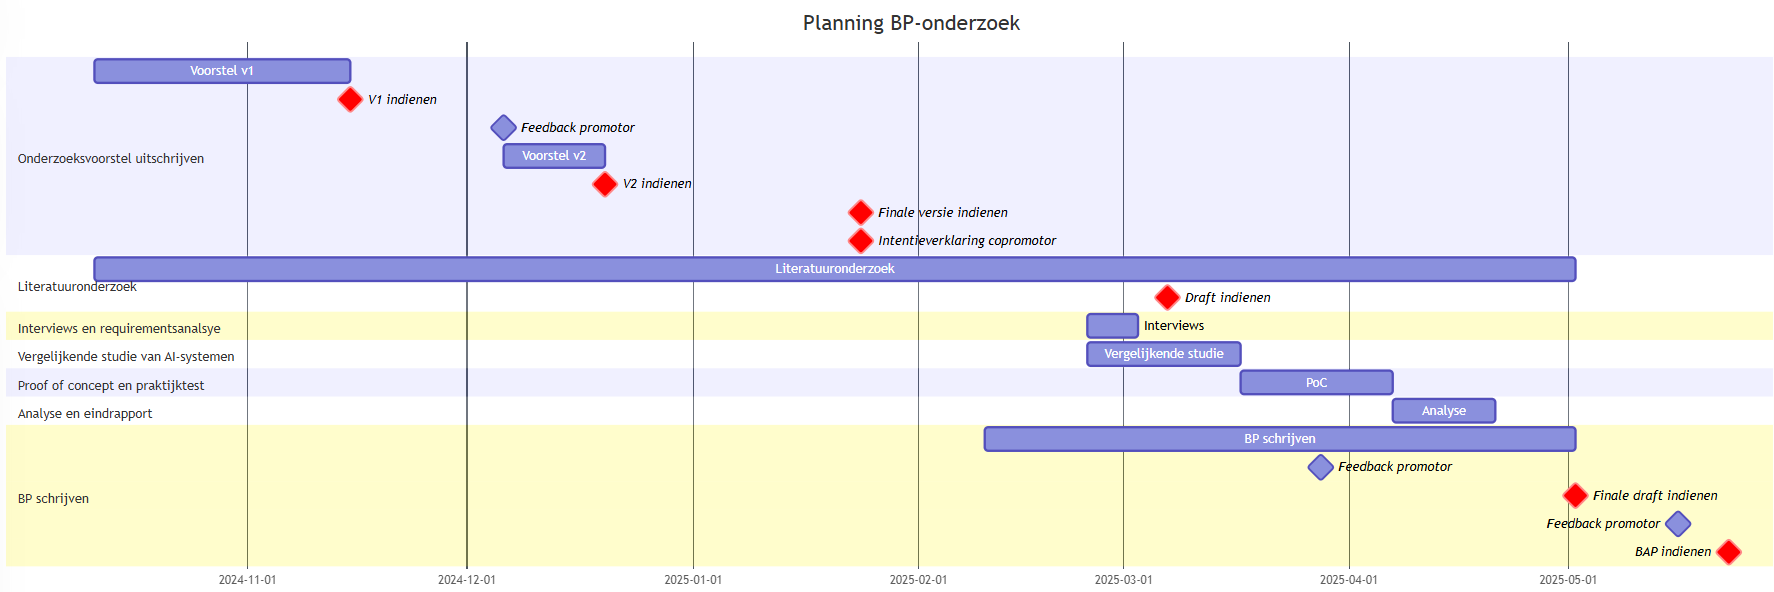
\includegraphics[width=0.5\textwidth]{img/gantt.png}
  \caption{\label{fig:gantt}Gantt planning bachelorproef}
\end{figure}

\begin{figure}[ht]
  \centering
  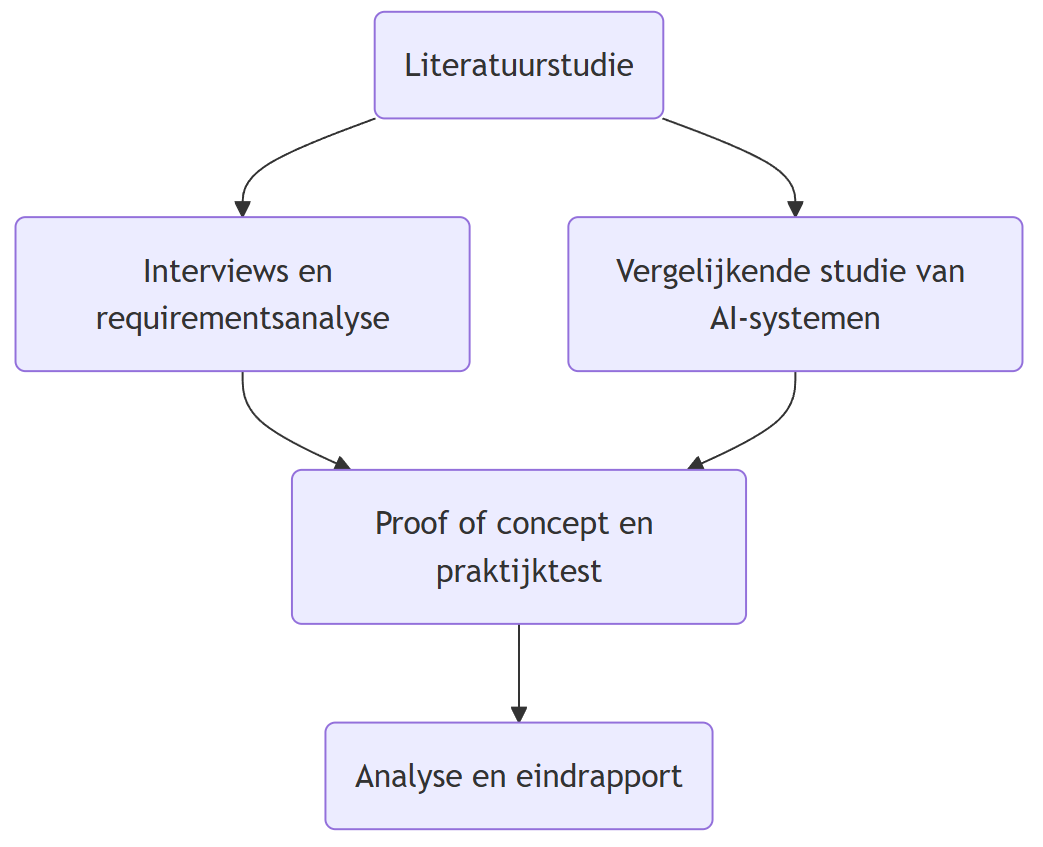
\includegraphics[width=0.3\textwidth]{img/flowchart.png}
  \caption{\label{fig:flowchart}Flowchart bachelorproef}
\end{figure}

%---------- Verwachte resultaten ----------------------------------------------
\section{Verwacht resultaat, conclusie}%
\label{sec:verwachte_resultaten}
Dit onderzoek richt zich op het automatiseren van spelers- en matchstatistieken bij volleybalclub Lindemans Aalst en beoogt een positieve invloed op de nauwkeurigheid en snelheid van dataverzameling, waarmee de club strategisch betere keuzes kan maken. Momenteel worden statistieken tijdens wedstrijden handmatig bijgehouden, terwijl er tijdens trainingen zelfs geen gegevens worden verzameld. Dit handmatige proces is tijdrovend en kan leiden tot inconsistenties in de data. Automatisering biedt potentieel voor een systeem dat in staat is realtime statistieken vast te leggen, zowel tijdens wedstrijden als trainingen, wat resulteert in een meer efficiënte en betrouwbare dataverzameling.

Allereerst wordt een verbetering verwacht in de nauwkeurigheid van gegevensverzameling. Het geautomatiseerde systeem zal naar verwachting 15-25\% nauwkeuriger zijn dan de handmatige methode door het verminderen van menselijke fouten.

Daarnaast wordt een aanzienlijke tijdsbesparing verwacht in de snelheid van data-analyse. Door een AI-gestuurd systeem toe te passen, kan de tijd voor gegevensverwerking en analyse met 30-50\% worden verminderd, wat vooral waardevol is tijdens het dynamische wedstrijdmoment. Het systeem maakt gegevens direct beschikbaar, zodat coaches en spelers tijdens wedstrijden hun beslissingen onmiddellijk kunnen aanpassen aan de realtime prestaties van het team.

Bovendien wordt verwacht dat het systeem de tactische beslissingen en trainingsinzichten van de coaches aanzienlijk zal verbeteren. Met de beschikbaarheid van gedetailleerde statistieken tijdens en na wedstrijden en trainingen zullen coaches in staat zijn om beslissingen te nemen op basis van een hogere kwaliteit en kwantiteit aan data.

De meerwaarde voor Lindemans Aalst ligt in drie hoofdgebieden: betere en snellere besluitvorming, efficiëntieverbetering en langetermijninzicht. Door realtime inzicht te krijgen in prestaties, zowel tijdens wedstrijden als trainingen, kunnen coaches gefundeerde keuzes maken, tijd besparen en diepgaandere analyses uitvoeren. Het systeem voegt waarde toe door historische gegevens op te slaan, waardoor coaches trends en de ontwikkeling van spelers effectief kunnen volgen. De resultaten van dit onderzoek bieden niet alleen een waardevolle tool voor Lindemans Aalst, maar verschaffen ook inzichten die andere sportorganisaties kunnen inspireren om AI-technologieën voor datagedreven analyse en besluitvorming te implementeren.
  
  \printbibliography[heading=bibintoc]

\end{document}